\chapter{Moje práce}
Tato práce třeba jednou bude hezká.

\section{Něco}
Aaargh.
\subsection{Menší něco}
Lalalalala. Chtěli bychom něco citovat. Tak třeba \cite{baker}.
\section{Ještě jedno něco}
Blalala. Kukni na obrazek~\ref{omnia.jpg}.


\pic{omnia.jpg}{Popis do seznamu obrazku.}{Dlooooooouhy popis, co bude pod obrázkem.}

\dpic{omnia.jpg}{skyrim.jpg}{seznamObrazkuOmnia}{popisDlouhyOmnia}{seznamObrazkuSkyrim}{popisDlouhySkyrim}

% \begin{figure}[H]
% \centering
% 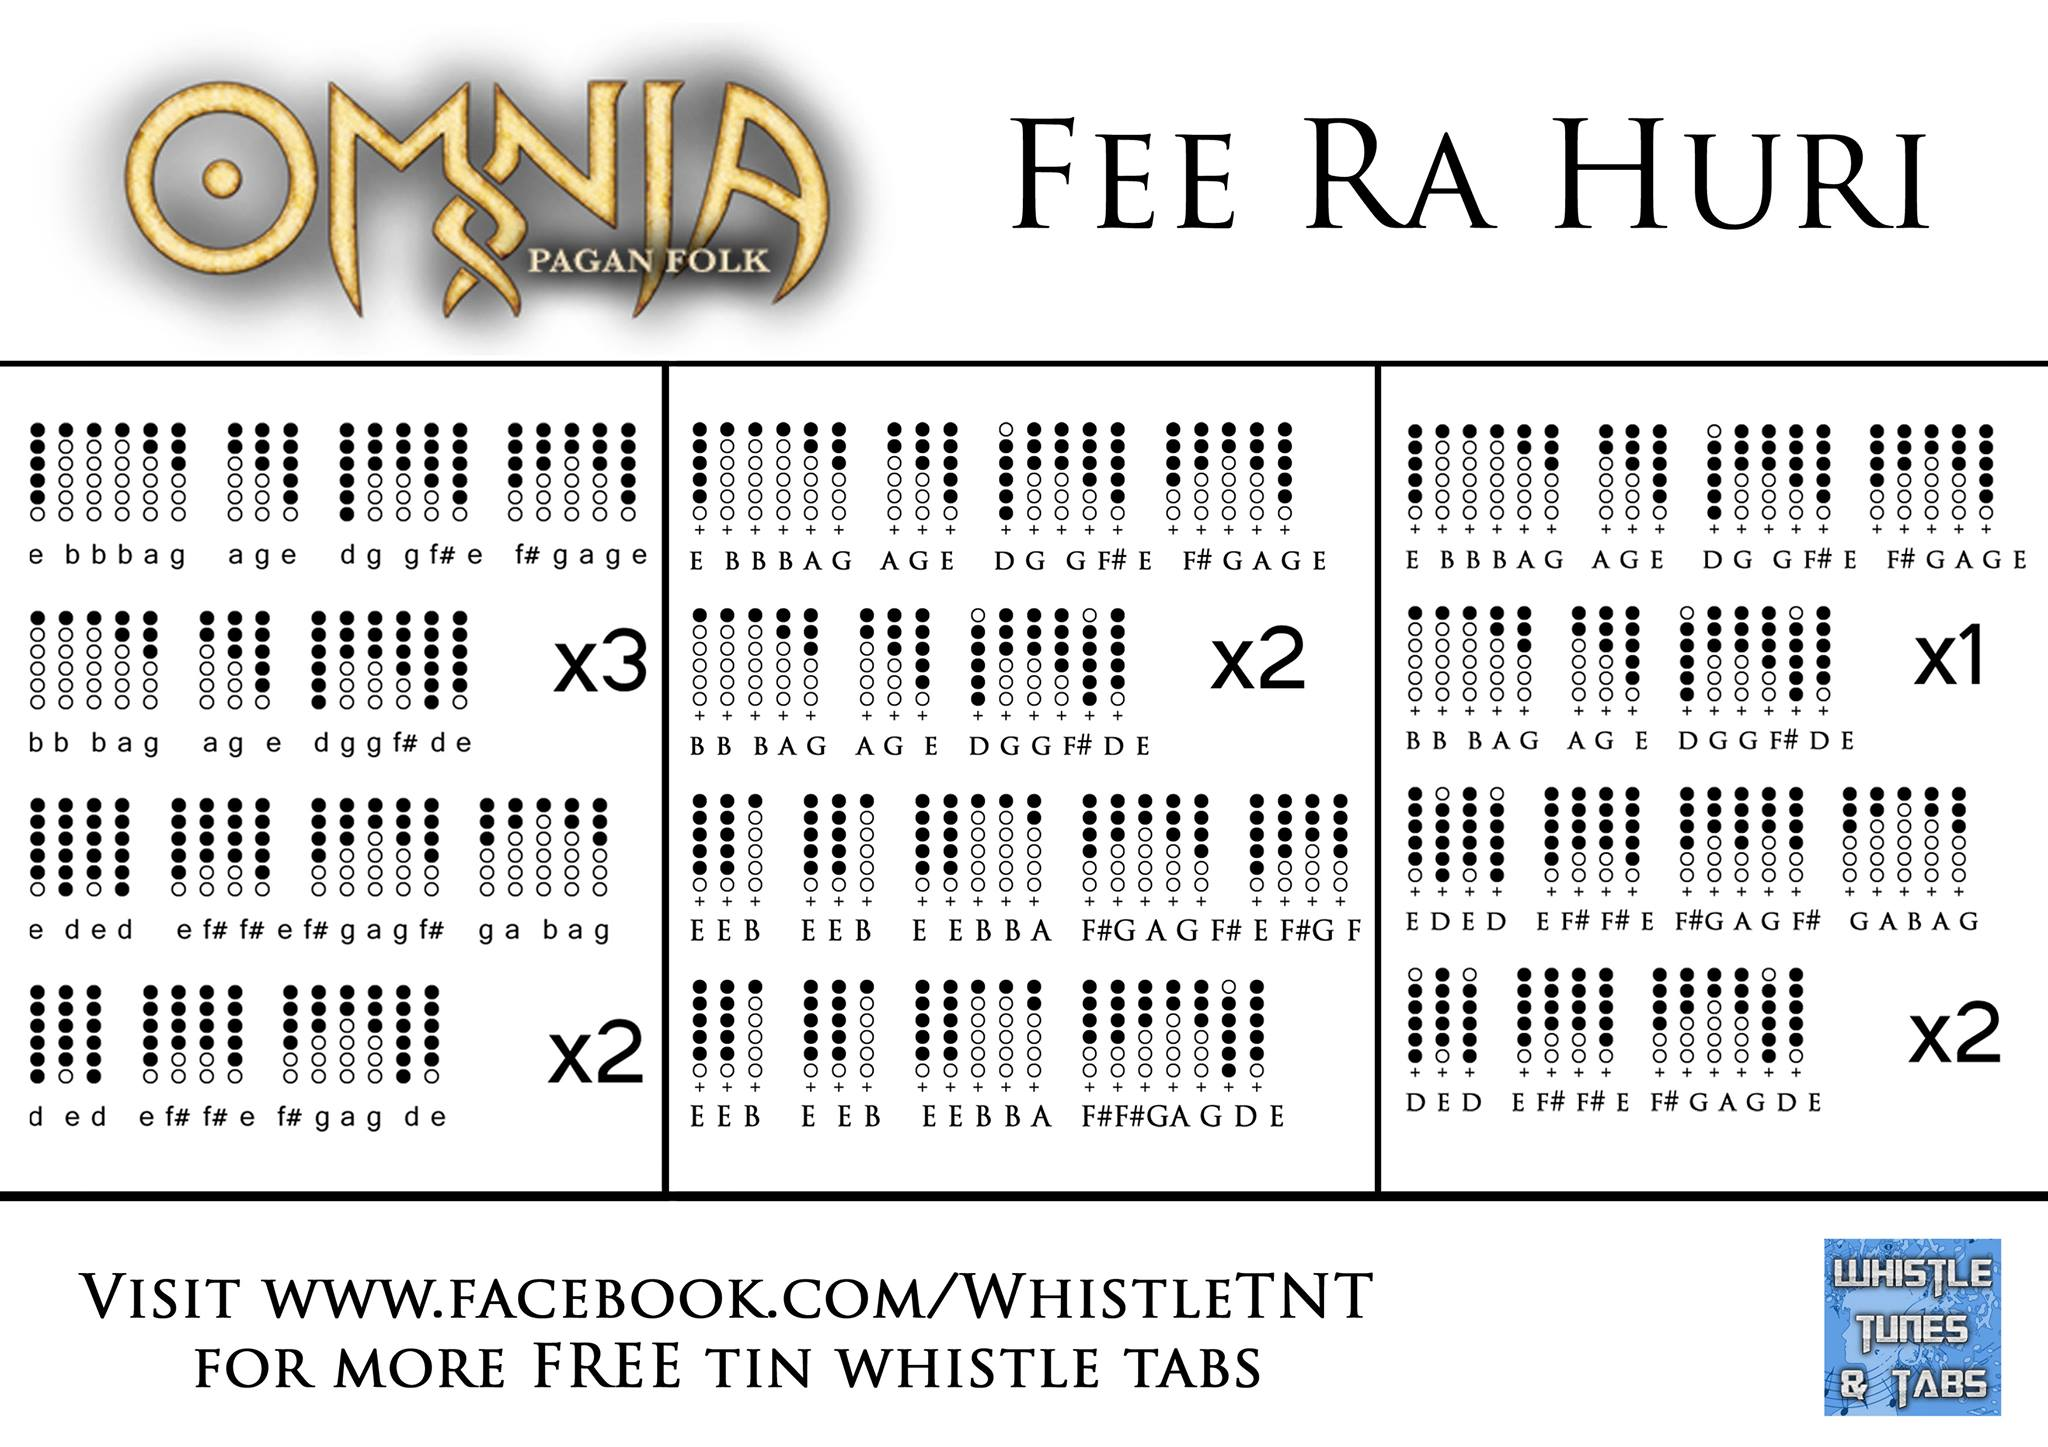
\includegraphics[width=0.8\textwidth]{./img/omnia.jpg}
% \caption[Popis do seznamu obrazku.]{Dlooooooouhy popis, co bude pod obrázkem.}
% \label{omnia.jpg}
% \end{figure}
% }
